\chapter*{Wstęp}
\label{cha:wstęp}

\section*{Wprowadzenie}
\label{sec:wprowadzenie}

Cyfrowe przetwarzanie sygnałów \ac{dsp} to dziedzina inżynierii, zajmująca się analizą, modyfikacją oraz optymalizacją sygnałów cyfrowych. Sygnały te mogą być wygenerowane cyfrowo lub przechodzić konwersję z postaci analogowej.
Przejście do cyfrowej formy sygnału miejsce, kiedy system wymaga operowania na sygnale dyskretnym reprezentowanym jako wartości liczbowe będące próbkami sygnału w czasie.

Przetwarzanie sygnałów znajduje szerokie zastosowanie w różnych dziedzinach technologii, w tym telekomunikacji (np. w systemach komunikacji mobilnej), audio (np. w korektorach dźwięku), bezpieczeństwa danych (np. w enkrypcji), medycynie (np. w diagnostyce) oraz w zastosowaniach militarncyh (np. w radarach i sonarch).
W kontekście telekomunikacji, \ac{dsp} daje nam możliwość przeprowadzania operacji modulacji i demodulacji, które odgrywają kluczową rolę w przesyle danych, umożliwiając efektywne kodowanie informacji oraz ich odczytanie po stronie odbiorczej. Ponadto, techniki takie jak redukcja szumów i zakłóceń są niezbędne do poprawy jakości sygnału.

Przetwarzanie sygnałów może odbywać się w różnych dziedzinach, takich jak czas, częstotliwość czy przestrzeń, co pozwala na szczegółową analizę i modyfikację sygnałów w zależności od zastosowania.
Transformacje takie jak \ac{fft} umożliwiają analizę sygnałów w dziedzinie częstotliwości, co jest kluczowe w przypadku systemów audio i wideo. Filtry \ac{dsp}, zarówno liniowe, jak i nieliniowe,
są używane do eliminacji zakłóceń, poprawy jakości dźwięku i obrazu oraz optymalizacji systemów transmisji danych.

\ac{dsp} daje nam możliwość tworzenie bardziej wydajnych systemów, które mogą przetwarzać coraz większe ilości danych w czasie. Zastosowania \ac{dsp} rozwijają się dynamicznie, obejmując coraz nowsze obszary,
od rozwoju sztucznej inteligencji po diagnostykę medyczną, co czyni tę dziedzinę niezbędną w rozwoju współczesnej technologii.

% \subsection*{Równoległe przetwarzanie danych}
% Algorytmy cyfrowego przetwarzania sygnałów (\ac{dsp}) stawiają wysokie wymagania wobec wydajności systemów obliczeniowych.
% Procesory, choć rozwijają się pod względem mocy obliczeniowej, napotykają ograniczenia wynikające z sekwencyjnego przetwarzania,
% co sprawia, że są mniej efektywne przy obliczeniach, które można prowadzić równolegle. W tym kontekście układy \ac{fpga} (Field-Programmable Gate Arrays) wyróżniają się
% możliwością równoległego przetwarzania danych, co pozwala na znaczne przyspieszenie złożonych operacji. Dzięki takiemu rozwiązaniu można przetwarzać wiele
% strumieni danych jednocześnie, co daje wyraźną przewagę nad procesorami, szczególnie w aplikacjach wymagających wysokiej przepustowości.

% \subsection*{Kontrola zegara i deterministyczne przetwarzanie}
% Kolejną zaletą układów \ac{fpga} jest możliwość precyzyjnego dostosowania częstotliwości zegara do wymagań projektowych. Dzięki wykorzystaniu języków opisu sprzętu,
% takich jak VHDL czy SystemVerilog, projektant ma pełną kontrolę nad wartościami sygałów w każdym takcie zegara, co umożliwia dokładne określenie, kiedy dane operacje mają się wykonywać.
% To daje pewność, że w takich aplikacjach jak filtr \ac{fir} dane będą przetwarzane i transmitowane w równych, określonych odstępach czasowych, co jest kluczowe. W odróżnieniu od procesorów,
% gdzie czas wykonywania kodu może być niedeterministyczny -- szczególnie w językach wysokiego poziomu, takich jak Python -- \ac{fpga} zapewniają
% pełną deterministyczność przetwarzania. Nawet w językach niskiego poziomu użytkownik nie zawsze ma pełną kontrolę nad czasem wykonywania kodu, ponieważ każda instrukcja wiąże się z pewnym narzutem czasowym.

\section*{Cel pracy}
\label{sec:cel_pracy}
% Część \ac{fpga} systemu jest odpowiedzialna za implementację
% algorytmów \ac{dsp}, zaś wbudowany procesor (HPS) pełni funkcję jednostki sterującej, uruchamiając serwer, który umożliwi użytkownikowi zdalną interakcję z systemem poprzez interfejs graficzny.

Celem niniejszej pracy była konstrukcja systemu do przetwarzania sygnałów cyfrowych opartego na układzie heterogenicznym (system łączący różne typy komponentów obliczeniowych). Kontrolę nad częścią systemu odpowiedzialną za \ac{dsp} według założeń miała pełnić aplikacja internetowa
umożliwiająca użytkownikowi zdalną interakcję z układem.

Motywacją do realizacji takiego projektu była chęć stworzenia w przyszłości platformy zdolnej do wydajnego przetwarzania sygnałów pochodzących z np. przetworników analogowo-cyfrowych (A/C) w czasie rzeczywistym. W wielu zastosowaniach przetwarzanie sygnałów
wymaga możliwości dostosowania architektury systemu do specyficznych potrzeb aplikacji, czego mogą nie oferować inne rozwiązania oparte np. o mikrokontrolery lub procesory \ac{dsp}. Ponadto dzięki integracji  układu \ac{fpga} z \ac{hps}, użytkownik ma możliwość zdalnego zarządzania
systemem oraz monitorowania przetwarzanych sygnałów, co zwiększa elastyczność i wygodę pracy. Umożliwia to szybkie dostosowywanie parametrów przetwarzania do konkretnych potrzeb, co jest istotne w wielu aplikacjach.

System ten ma na celu nie tylko zaprezentowanie w praktyce możliwości przetwarzania sygnałów, ale również stworzenie podstawy do dalszego rozwoju o kolejne funkcjonalności, takie jak implementacja nowych algorytmów \ac{dsp}, rozszerzenie interfejsu użytkownika,
czy integracja z innymi systemami przetwarzania danych.
% Część \ac{fpga} systemu będzie odpowiedzialna za implementację algorytmów \ac{dsp}, w tym filtru \ac{fir} oraz modułu
% realizującego dyskretną transformatę Fouriera (DFT). System ten będzie wyposażony w dwie pamięci, pomiędzy którymi dane będą transmitowane, przetwarzane, a następnie zapisywane.
% Równocześnie wbudowany procesor będzie pełnił funkcję jednostki sterującej, uruchamiając serwer, który umożliwi użytkownikowi zdalną interakcję z systemem poprzez stronę internetową.
% Strona będzie umożliwiać wprowadzanie danych do FPGA, inicjowanie procesów przetwarzania oraz monitorowanie wyników. Taki podział zadań na układ \ac{fpga} i HPS umożliwia
% efektywną realizację algorytmów \ac{dsp}, zapewniając wysoką wydajność oraz intuicyjną obsługę przez użytkownika.

\section*{Zakres pracy}
\label{sec:zakresPracy}
Zakres pracy obejmował opracowanie systemu umożliwiającego przesył i odczyt danych pomiędzy \ac{hps} a pamięciami w \ac{fpga}, a także transmisję tych danych z wkorzystaniem \ac{dma} między obiema pamięciami.

Oprócz tego, praca skupi się na opracowaniu i implementacji w systmie filtru \ac{fir} umożliwiającego modyfikację współczynników w trakcie pracy, co zapewni większą elastyczność przetwarzania danych. System będzie również wykorzystywał moduł \ac{fft} będący IP Quartusa,
który umożliwi podgląd przetworzonych sygnałów w dziedzinie częstotliwości.

W ramach pracy powstanie również strona internetowa, która pozwoli użytkownikowi na przesył danych, komunikację z systemem oraz wizualizację wyników. Interfejs strony zostanie zaprojektowany z myślą o intuicyjnej obsłudze,
a także w sposób umożliwiający łatwą implementację kolejnych funkcjonalności w przyszłości.

\section*{Struktura pracy}
\label{sec:strukturaPracy}


% \subsection{Platforma Cyclone V SoC}
% W mojej pracy skupię się na układzie heterogenicznym \ac{fir}my Intel -- Cyclone V SoC. Jest to budżetowy układ zawierający w swojej architekturze zarówno FPGA, jak i
% HPS (Hard Processor System) oparty na procesorze ARM, co pozwala na rozdzielenie zadań pomiędzy obie architektury. Mimo że Cyclone V SoC nie jest układem najwyższej klasy,
% jego cena oraz możliwości konfiguracyjne sprawiają, że znajduje zastosowanie w projektach wymagających kompromisu między wydajnością a kosztami. W mojej pracy pokażę, jak można
% efektywnie wykorzystać ten układ do implementacji zaawansowanych algorytmów przetwarzania sygnałów.

% \begin{figure}[!htb]
%     \centerline{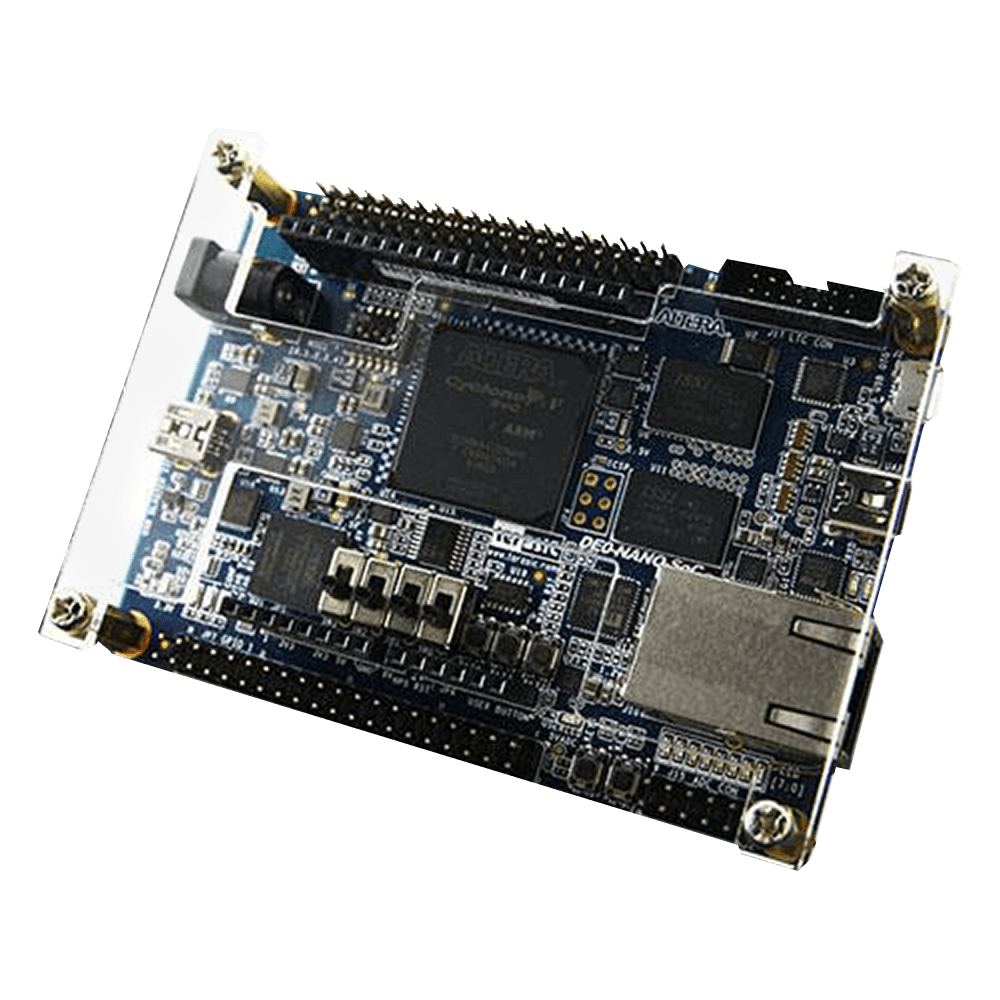
\includegraphics[scale=0.2]{de0-nano-soc.png}}
%     \caption{Układ DE0-Nano-SoC (Cyclone V)}
%     \label{fig:de0-nano-soc}
% \end{figure}



















